\documentclass[12pt]{article}

\title{Theory of computation\\ Practical Assignment 2}
\author{Jason Naldi, Ha Minh, Valdet, Ismaili,\\ Georgios Koursiounis, Luka Volk}

\usepackage{amsmath}    % need for subequations
\usepackage{graphicx}   % need for figures
\usepackage{verbatim}   % useful for program listings
\usepackage{color}      % use if color is used in text
\usepackage{subfigure}  % use for side-by-side figures
\PassOptionsToPackage{hyphens}{url}
\usepackage{hyperref}
\usepackage{gensymb}
\usepackage[utf8]{inputenc}


\begin{document}
\maketitle

\section{Introduction}
\subsection{Definition of Complete Graphs}

In the mathematical field of graph theory, a complete graph is a simple undirected graph in which every pair of distinct vertices is connected by a unique edge. A complete graph $K_n$ with $n$ vertices has $\binom{n}{2}\frac{n(n-1)}{2}$ undirected edges \footnote{\url{https://en.wikipedia.org/wiki/Complete\_graph}}.

\begin{figure}[ht!]
    \centering
    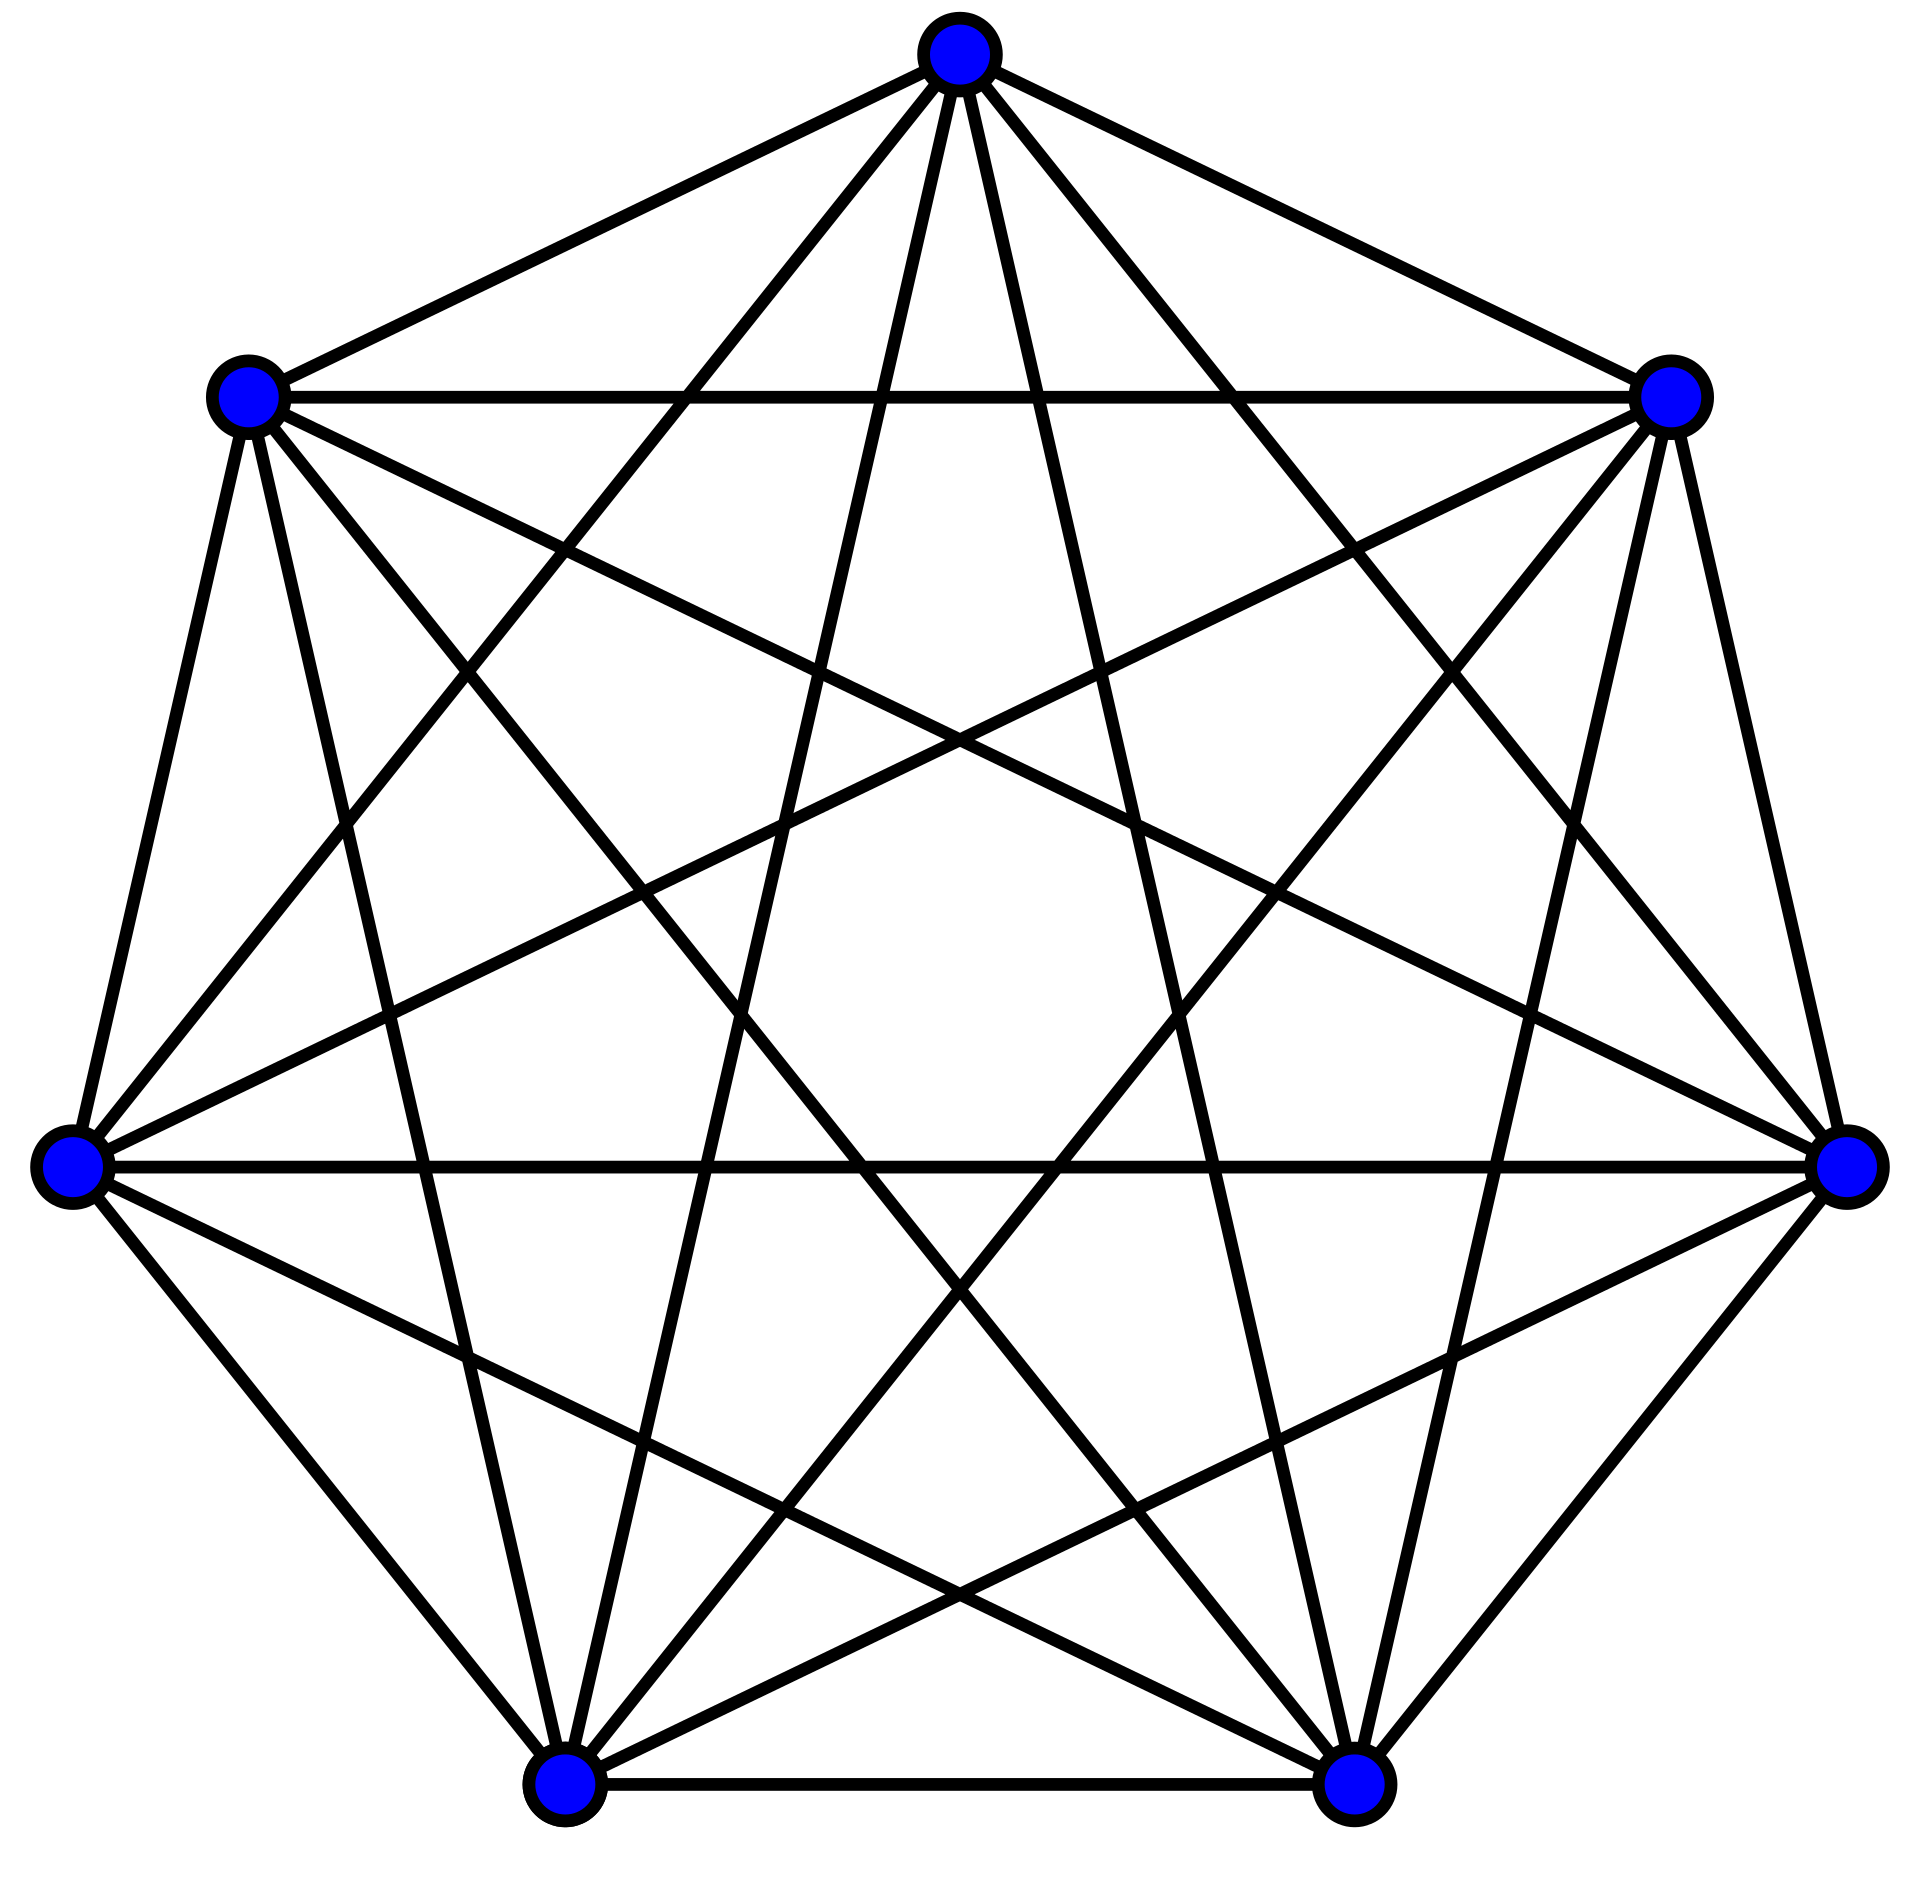
\includegraphics[width=5cm, height=5cm]{Complete_graph.png}
    \caption{Example of Complete Graph}
\end{figure}

\subsection{K-clique problem description}

A clique in an undirected graph is a sub-graph, where in every two nodes are connected by an edge. A k-clique is a clique that contains k nodes
\footnote{Introduction to the Theory of Computation, Sipser, 3rd edition, p.295}
and can be written in mathematical form as follows:

\begin{center}
$CLIQUE = \{<G, k> | G$ is an undirected graph with a k-clique\}
\end{center}

The clique problem is to determine whether a graph contains a clique of a specified size $k$. That problem ofter arises in many aspects of the digital age. Consider a social network, where the graph's vertices represent people, and the graph's edges represent mutual acquaintance. Then a clique represents a subset of people who all know each other, and algorithms for finding cliques can be used to discover these groups of mutual friends
\footnote{\url{https://en.wikipedia.org/wiki/Clique\_problem}}. From theory, we also know that $CLIQUE$ is NP-Complete.

\begin{figure}[ht!]
    \centering
    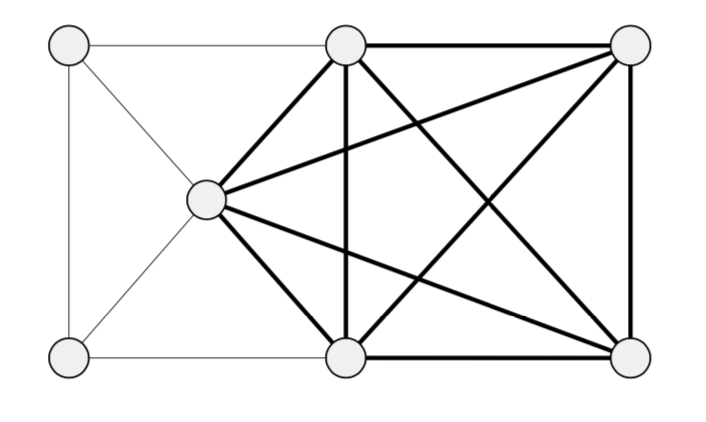
\includegraphics[width=7cm, height=4cm]{5clique.png}
    \caption{A graph which contains a 5-clique}
\end{figure}


\section{Redution}

Let $G(V,E)$ be a graph, where $V$ is a list of vertices and $E$ is a list of edges connecting two vertices of $V$ each. Then, let $k$ be the size of the desired clique.

Let $C$ be a clique of size $k$ in $G$. This clique is represented as a list of $k$ vertices, where the $i$th element of $C$ is the $i$th vertex in the clique.

Let $x_{i,v}$ be a boolean variable for every pair $(i,v)$, where $i \in (1, k)$ and $v \in V$. Then, each variable $x_{i,v}$ indicates whether vertex $v$ is the $i^{th}$ vertex in the clique.

Then, it is easy to compose a CNF statement that is true only if there exists a clique of size $k$ in $G$. The conditions are:

\begin{itemize}
  \item every vertex in the clique must be unique (i.e. each vertex $v$ in $V$ can appear at most once in the clique)
  \item if two vertices $v_1$ and $v_2$ do not share an edge, then they both cannot be part of the clique
  \item each position $i$ in the clique can hold exactly one vertex $v \in V$ only.
\end{itemize}

More formally:

\begin{itemize}
  \item for each two positions $i,j \in 0 \dots k$ in the clique $C$, if $i \neq j$ then it must hold that $x_{i,v} \neq x_{j,v}$
  \item for each two vertices $v, w \in G$ which are not connected by an edge $e \in E$, both $v$ and $w$ cannot be in the clique $C$
  \item for each position $i \in 0 \dots k$ in the clique $C$, the size of the set $\{v_{i,v} \, | \, v \in V \and v_{i,v} \in C\}$ is exactly $1$.
\end{itemize}

Expressed as CNF:

\begin{itemize}
  \item for each $i \in 0 \dots k\,: \bigvee_{v \in V} x_{i,v}$
  \item for each $i,j \in 0 \dots k$ where $i \neq j$, and for each $v \in V$: $\lnot x_{i,v} \lor \lnot x_{j,v}$
  \item for each $i,j \in 0 \dots k$ where $i \neq j$, and for each two vertices $v$, $w$ where no edge $e \in E$ connecting $v$ and $w$ exists and $v \neq w$: $\lnot x_{i,v} \lor \lnot x_{j,w}$
  \item for each $i \in 0 \dots k$ and for each two vertices $v$, $w$ where $v \neq w$: $\lnot x_{i,v} \lor \lnot x_{i,w}$
\end{itemize}

\section{Implementation}

The attached script \texttt{reduction.py} takes as input as file with the following structure:

\begin{verbatim}
  size_k_of_clique number_of_vertices_in_graph
  adjacency_list
\end{verbatim}

where the adjacency list is a list of newline separated pairs of nodes, each pair of nodes separated by an empty space. (See included \texttt{example\_input.txt} for a template input.)

The attached python3 script takes care of
\begin{enumerate}
  \item reading the input
  \item composing the adjacency matrix of the given graph
  \item produce the CNF formula for the requested clique size and given graph (in DIMACS format)
  \item feed the CNF formula to \texttt{minisat}
  \item output either \texttt{UNSAT} if no clique of size $k$ exists for the given graph or the list of nodes in the clique separated by new line if the clique exists. Note that the program will also create a PNG file containing a visual representation of the graph with the clique's edges highlighted in red. The visualisation requires having \texttt{graphviz} installed on the machine.
\end{enumerate}

The script requires one command-line arguments: the path of the input file.

\end{document}
